% !TeX root = ./main.tex

\documentclass[12pt]{article}
\usepackage{graphicx}
\usepackage{float}
\usepackage[a4paper, margin=1in]{geometry}

\title{Progress in Screening Methodology}
\author{Shlok Mishra}
\date{\today}

\begin{document}

\maketitle

\section{Example 1. A location problem with marginal features}
I made the modification of changing the median of the signals to 5 in order to improve the performance of the screening algorithm.\\
In 100/100 cases, the set of detected signals is exactly equal to the actual set. The actual set of marginals is \{1, 2, 3, 4\}.\\
Here is the barplot which portrays how many times each feature was detected using our screening algorithm.
\begin{figure}[H]
    \centering
    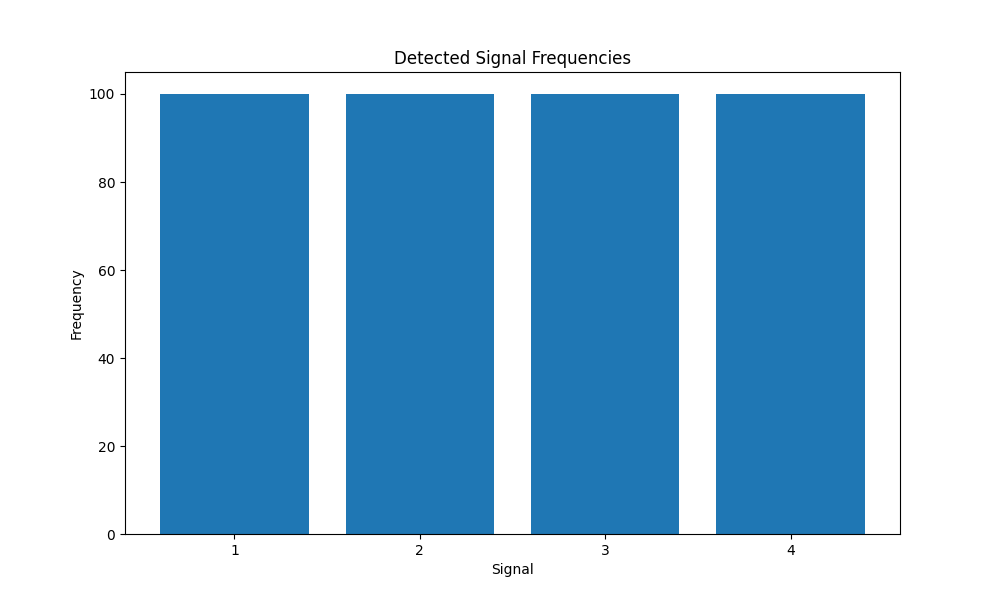
\includegraphics[width=0.6\textwidth]{eg1.png}
    \caption{Frequency of different features in detected signals for Example 1}
\end{figure}

\section{Example 2. A scale problem with paired features.}
I made no modifications to the example.\\
In 100/100 cases, the correct set of signal pairs \{1,2\} and \{3,4\} is exactly detected in the pair column. \\
Here is the barplot which portrays how many times each pair of features was detected using our screening algorithm.
\begin{figure}[H]
    \centering
    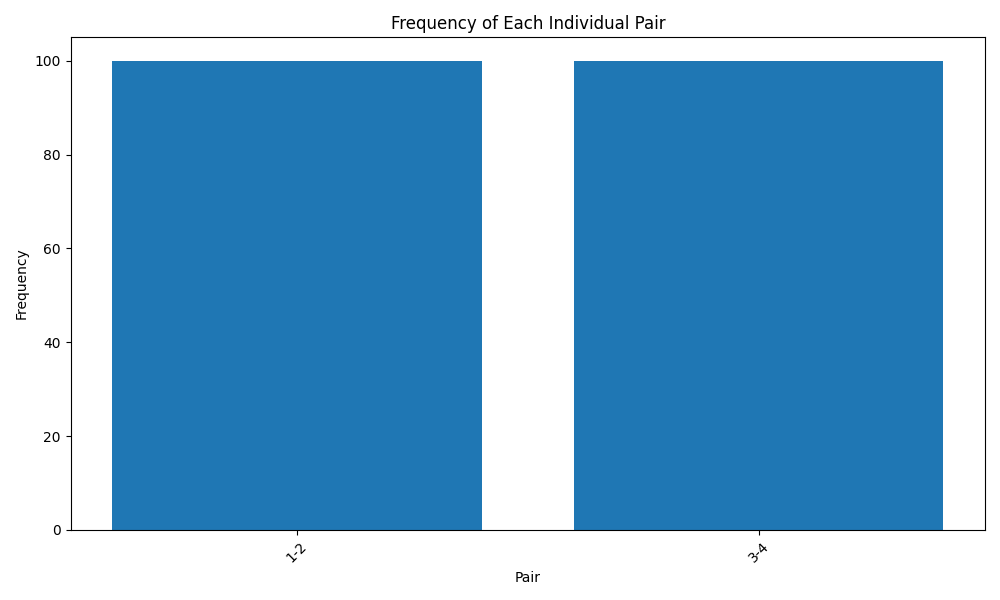
\includegraphics[width=0.6\textwidth]{eg2.png}
    \caption{Frequency of detected signal pairs for Example 2.}
\end{figure}
\section{Example 3. A location-scale problem with marginal and paired features}
We are yet to build a screening algorithm to deal with such mixed cases.
% \begin{figure}[H]
%     \centering
%     \includegraphics[width=0.6\textwidth]{eg3.png}
%     \caption{Frequency of different features in detected signals for Example 3.}
% \end{figure}

\section{Example 4. A scale problem with marginal features}
I made the modification of changing the scaling factor to 10 in order to improve the performance of the screening algorithm.\\
In 85/100 cases, the set of detected signals is exactly equal to the actual set. The actual set of marginals is \{1, 2, 3, 4\}.\\
Here is the barplot which portrays how many times each feature was detected using our screening algorithm.
\begin{figure}[H]
    \centering
    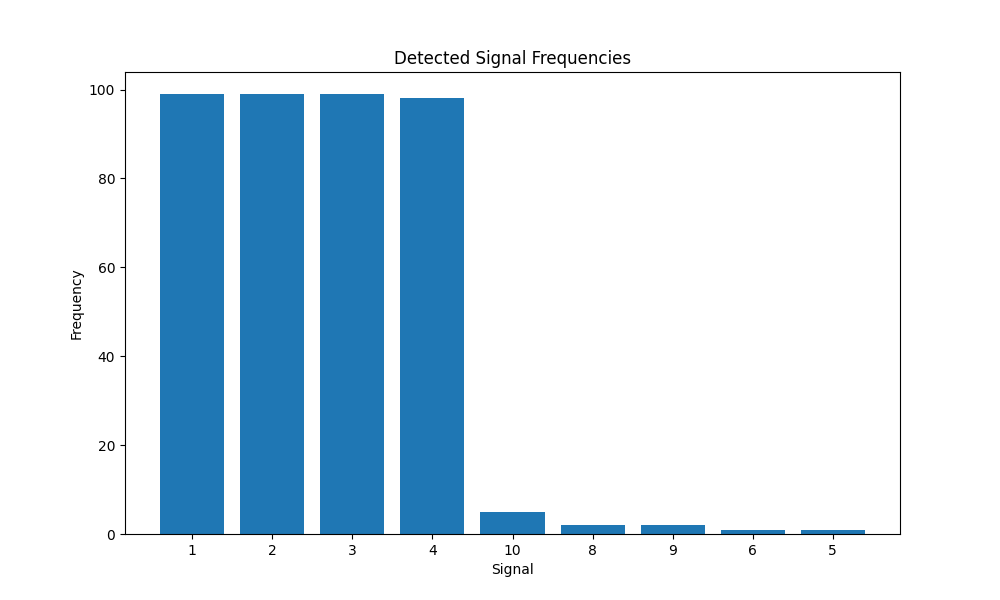
\includegraphics[width=0.6\textwidth]{eg4.png}
    \caption{Frequency of different features in detected signals for Example 4.}
\end{figure}

\section{Example 5. A heavy-tailed location problem with marginal features.}
I made no modifications to the example.\\
In 98/100 cases, the set of detected signals is exactly equal to the actual set. The actual set of marginals is \{1, 2, 3, 4\}.\\
Here is the barplot which portrays how many times each feature was detected using our screening algorithm.
\begin{figure}[H]
    \centering
    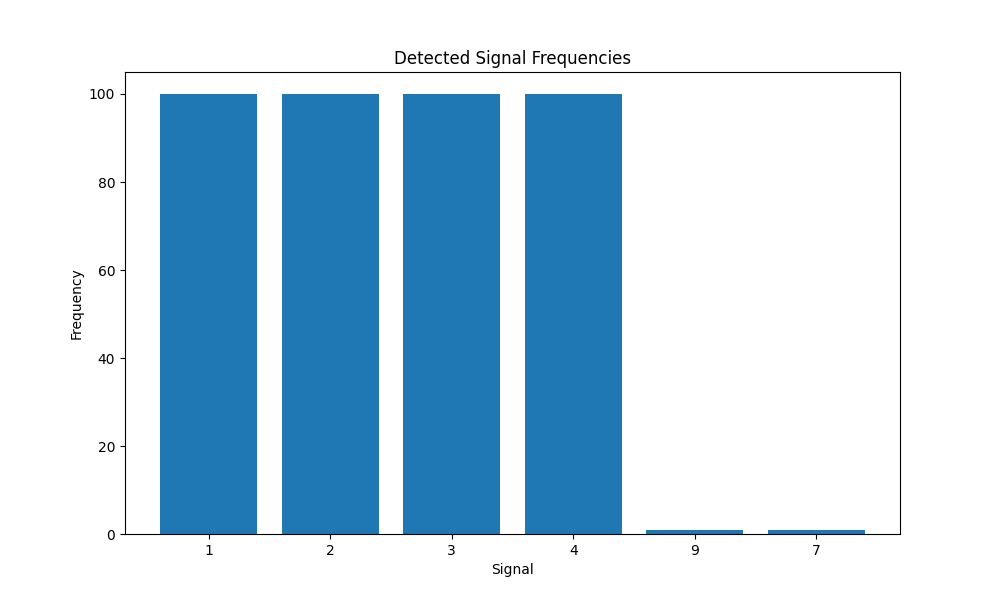
\includegraphics[width=0.6\textwidth]{eg5.png}
    \caption{Frequency of different features in detected signals for Example 5.}
\end{figure}

\section{Example 6. A heavy-tailed scale problem with marginal features.}
I made the modification of changing the scaling factor of Cauchy distribution to 10 in order to improve the performance of the screening algorithm.\\
In 91/100 cases, the set of detected signals is exactly equal to the actual set. The actual set of marginals is \{1, 2, 3, 4\}.\\
Here is the barplot which portrays how many times each feature was detected using our screening algorithm.
\begin{figure}[H]
    \centering
    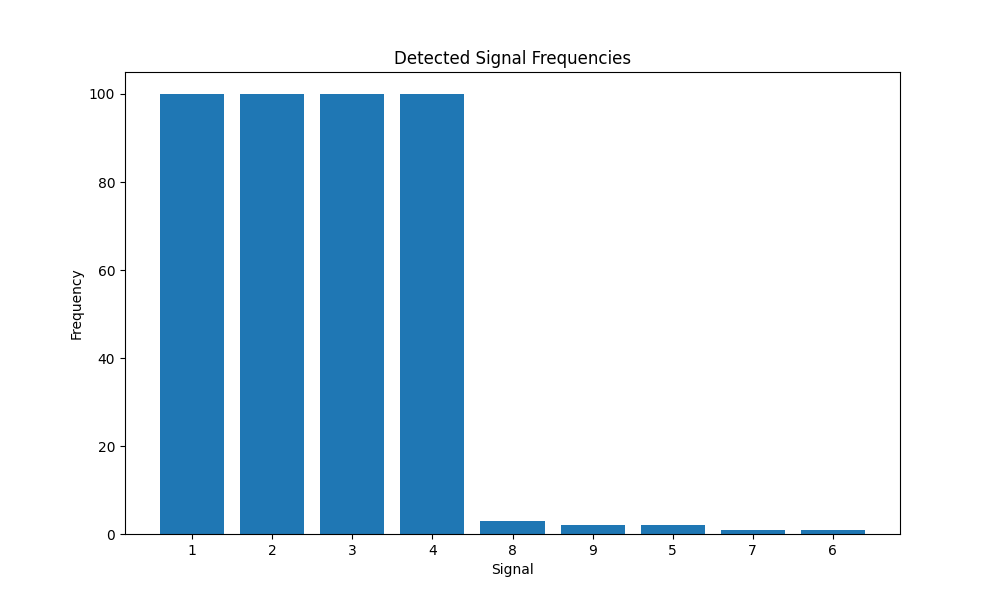
\includegraphics[width=0.6\textwidth]{eg6.png}
    \caption{Frequency of different features in detected signals for Example 6.}
\end{figure}

\section{Example 7. A location-scale problem with mixture distributions having marginal features.}
I made the modification of changing the variance of noise to 0.1 in order to improve the performance of the screening algorithm.\\
In 81/100 cases, the set of detected signals is exactly equal to the actual set. The actual set of marginals is \{1, 2, 3, 4\}.\\
Here is the barplot which portrays how many times each feature was detected using our screening algorithm.
\begin{figure}[H]
    \centering
    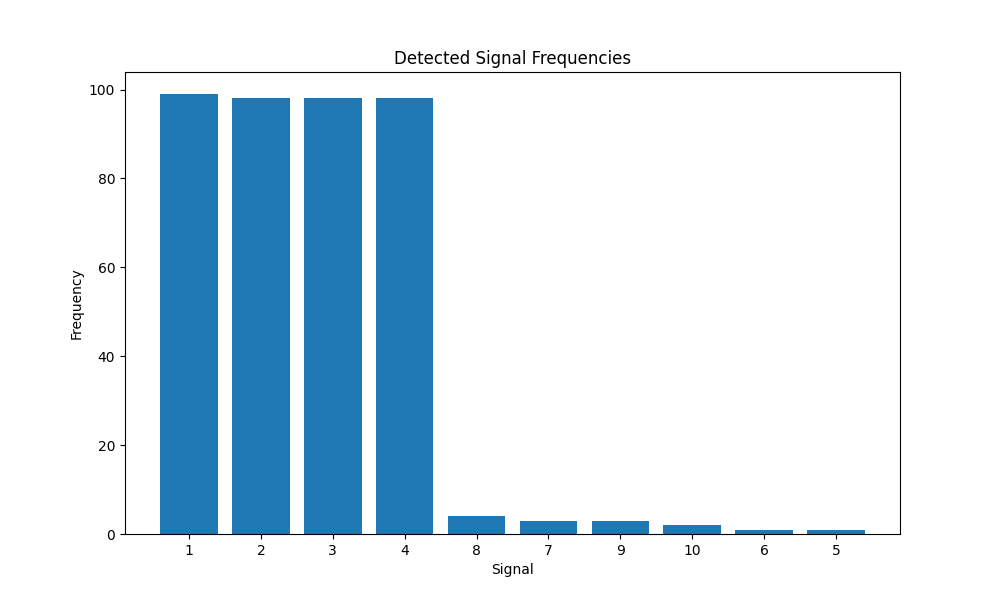
\includegraphics[width=0.6\textwidth]{eg7.png}
    \caption{Frequency of different features in detected signals for Example 7.}
\end{figure}

\section{Example 8. A scale problem with paired features.}
I made the modification of changing the variance of noise to 0.01 in order to improve the performance of the screening algorithm.\\
In 64/100 cases, the correct set of signal pairs \{1,2\} and \{3,4\} is exactly detected in the pair column. \\
Here is the barplot which portrays how many times each pair of features was detected using our screening algorithm.
\begin{figure}[H]
    \centering
    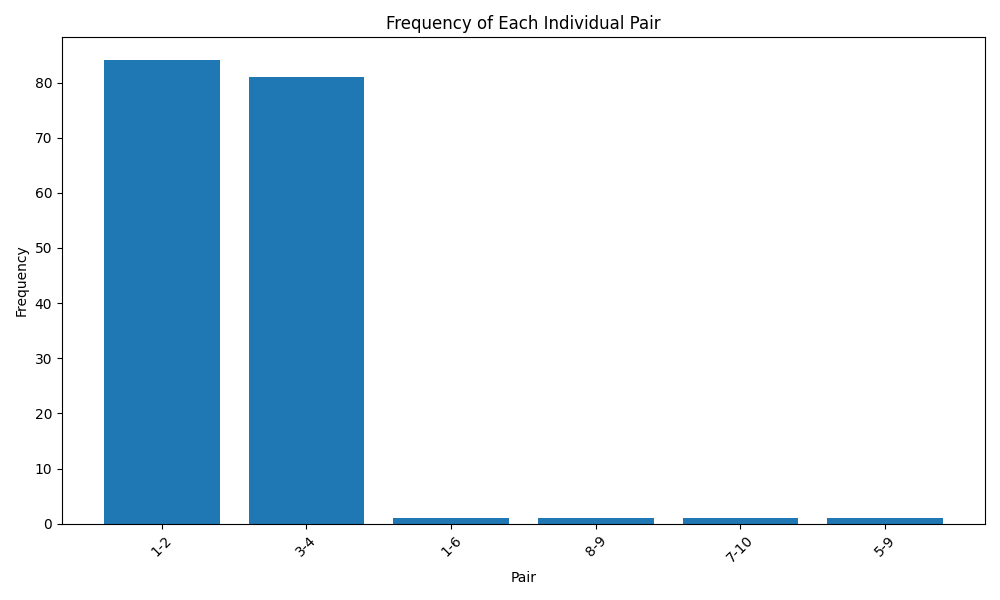
\includegraphics[width=0.6\textwidth]{eg8.png}
    \caption{Frequency of detected signal pairs for Example 8.}
\end{figure}

\section{Misclassification Rates of Each Example}

The following table presents the misclassification rates for each example as percentages, based on average of 100 trials:

\begin{table}[H]
    \centering
    \begin{tabular}{|c|c|c|}
        \hline
        \textbf{Example} & \textbf{Classifier Used} & \textbf{Misclassification Rate (\%)} \\
        \hline
        Example 1        & MarKS                    & 0\%                                  \\
        Example 2        & PairKS                   & 5.264\%                                \\
        Example 3        & MixKS                    & N/A                                  \\
        Example 4        & MarKS                    & 7.454\%                               \\
        Example 5        & MarKS                    & 24.246\%                               \\
        Example 6        & MarKS                    & 14.594\%                               \\
        Example 7        & MarKS                    & 3.756\%                                \\
        Example 8        & PairKS                   & 26.472\%                              \\
        \hline
    \end{tabular}
    \caption{Average Misclassification Rates as Percentages for Each Example}
\end{table}

\end{document}
